\documentclass[border=3pt]{standalone}
\usepackage[T1]{fontenc}
\usepackage{lmodern}
\usepackage{amsmath,amssymb}
\usepackage{tikz}
\usepackage{pgfplots}
\pgfplotsset{compat=1.17}
\usepgfplotslibrary{groupplots}
\usetikzlibrary{arrows.meta,calc,positioning,fit,backgrounds}

% Autonomous vehicle: camera, LiDAR and radar fused for detection, tracking and planning.
\begin{document}
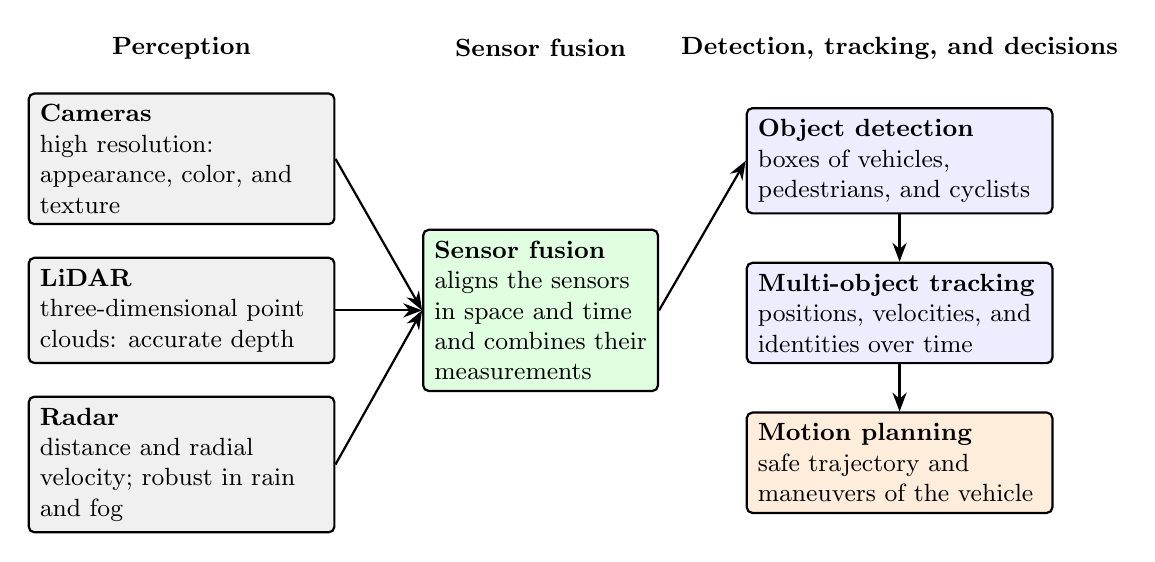
\begin{tikzpicture}[
  font=\small,
  sen/.style={draw, thick, rounded corners=2pt, align=flush left, text width=36mm, inner sep=4pt,
              minimum height=13mm, fill=gray!12},
  proc/.style={draw, thick, rounded corners=2pt, fill=blue!7, align=flush left, text width=36mm, inner sep=4pt},
  fus/.style={draw, thick, rounded corners=2pt, fill=green!12, align=flush left, text width=27mm, inner sep=4pt},
  res/.style={draw, thick, rounded corners=2pt, fill=orange!14, align=flush left, text width=36mm, inner sep=4pt},
  arr/.style={-{Stealth[length=2.4mm]}, thick},
  hdr/.style={font=\small\bfseries, align=center}]
% sensors
\node[sen] (cam) at (0,0) {\textbf{Cameras}\\ high resolution: appearance, color, and texture};
\node[sen, below=4mm of cam] (lid) {\textbf{LiDAR}\\ three-dimensional point clouds: accurate depth};
\node[sen, below=4mm of lid] (rad) {\textbf{Radar}\\ distance and radial velocity; robust in rain and fog};
% fusion
\node[fus, right=11mm of lid] (fu) {\textbf{Sensor fusion}\\ aligns the sensors in space and time and combines their measurements};
% detection, tracking, planning
\node[proc, right=11mm of fu, yshift=19mm] (det) {\textbf{Object detection}\\ boxes of vehicles, pedestrians, and cyclists};
\node[proc, below=6mm of det] (trk) {\textbf{Multi-object tracking}\\ positions, velocities, and identities over time};
\node[res, below=6mm of trk] (pln) {\textbf{Motion planning}\\ safe trajectory and maneuvers of the vehicle};
% arrows
\foreach \s in {cam, lid, rad} \draw[arr] (\s.east) -- (fu.west);
\draw[arr] (fu.east) -- (det.west);
\draw[arr] (det) -- (trk);
\draw[arr] (trk) -- (pln);
% column headers
\node[hdr, above=3mm of cam] (h1) {Perception};
\node[hdr] at (fu |- h1) {Sensor fusion};
\node[hdr] at (det |- h1) {Detection, tracking, and decisions};
\end{tikzpicture}
\end{document}
